% +--------------------------------------------------------------------+
% | Sample Chapter
% |
% | This file provides examples of how to
% | - insert a figure with a caption
% | - construct a table with a caption
% | - create subsections within the chapter
% | - insert a reference to a Figure or Table
% | - make a citation
% +--------------------------------------------------------------------+

\cleardoublepage

% +--------------------------------------------------------------------+
% | Replace "Chapter Title" below with the title of your chapter.  LaTeX
% | will automatically number the chapters.
% +--------------------------------------------------------------------+

\chapter{Introduction}
%\label{ch:Introducción}
\label{makereference}


% +--------------------------------------------------------------------+
% | Replace \section headings below with the title of your
% | subsections.  LaTeX will automatically number the subsections 1.1,
% | 1.2, 1.3, etc.
% +--------------------------------------------------------------------+

\section{Motivation}
\label{makereference1.1}

{\em Cloud computing} has been a major word speaking about data compute in the last decade; as of today, cloud computing is used to store, clean, process and analyze virtually every chunk of information gathered from any source.
%
With the emergence of Internet of Things (IoT), cloud computing is still a hot topic and an integral part in the deployment of complete infrastructures, prividing easy and scalable access to applications, resources and services, and being fully managed by  cloud service providers~\cite{cloud_def}.

IoT devices provide large amount of data, and hence cloud processing is a natural solution to deal with them. 
%
The {\em Cloud of Things} (CoT) term comes here into play,  deploying connected defices directly to the cloud to perform complex operations with the generated data using with Artificial Intelligence. This is the perfect tool for creating smart tasks that harness the immense amount of information.
%
However, Cloud Computing faces several challenges to meet the most stringent performance requirements of many application services, specially in terms of latency and bandwidth~\cite{IEE:Morabito:2017}.

To address and solve those problems, Edge Computing is a new paradigm that aims at bringing data storage and computation closer to the data source in order to improve response times and save data bandwidth. Edge Computing consists on increasing the resources available on the network edge, adopting a platform that provides intermediate layers for storing, cleaning, analyzing and inferencing.
%
Regarding the layers located at the edge, it is obviously impossible to provide the same kind of datacenter capabilities that are currently available in Cloud Computing premises. Edge Computing implies limited computational capabilities, so one of the main problems to be solved is to get similar cloud platforms (at least in terms of capabilities, flexibility and deployment mechanisms) into an edge environment with certain compute power for processing data.

Specifically, an edge computing infrastructure is based on a set of local hardware resources, that we have also adopted in this work. Specifically, we base our development on a fairly common hardware infrastructure composed of two main elements, namely:

\begin{itemize}
  \item \textbf{A Single Board Computer (SBC) or a minicomputer/barebone} that exhibit relatively high computing capacities with a proper reducing cost, energy consumption and form factor to adapt it to the specific scenario in which they are usually deployed.
  \item \textbf{Specific-purpose USB accelerators (DSAs)}, that provide co-processing capabilities to the central aforementioned computer (e.g. an Edge TPU as a Machine-Learning coprocessor). It accelerates specific tasks (e.g. inference processes for artificial intelligence models in the case of the Edge TPU), and can be selected depending on the typical application types that will be deployed on the edge infrastructure.
\end{itemize}

While the hardware problem is covered with the aforementioned elements, 
there are other elements involving the current paradigm of Cloud and Edge computing that are critical in order to develop an efficient and flexible edge architecture. 

\textbf{Virtualization} is the capability of creating virtual machines that act like real ones. This technology becomes mandatory in Cloud and Cdge Computing, since the creation of automatic elastic services requires getting rid of haphazard IT rooms, cables, and bulky hardware, reducing the overall IT overhead as well as management costs~\cite{virt_def}.

The creation and management of these virtual machines (VMs) would be impossible without the existence of \textbf{hypervisors}, pieces of software in charge of controlling the VM and providing a connection for the virtual resource and the real one.

\textbf{Virtual appliances} are VM images, usually with a specific configuration, designed to run on a virtual platform. They are designed to reduce or eliminate the installation, configuration, and maintenance costs associated with running suites of software~\cite{GEN:Virtualization:2010}.

When anything is able to connect to the Internet and generate data, there will be a possibility that at some stage uploading data to the cloud or sync device won't be necessary any longer. Temporarily, the data might not be required. In that scenario, either the device must be stopped from generating data or gateway device must decide when the data upload should be discontinued to avoid using network and cloud resources for a while.~\cite{Ficloud:AazaamHuh:2014}
Having this in mind and knowing that in a near future there are going to be millions devices called things connected, the \textbf{IoT gateway} appears to serve as a bridge for connecting these things, send data to the cloud or participate with an edge approach. A way to implement this edge gateway might be building a virtual appliance that will be situated close to the things. Figure ~\ref{figure1.1} shows a representation of the concept.


\newpage
\begin{figure}[h]%t=top, b=bottom, h=here
% \centering
    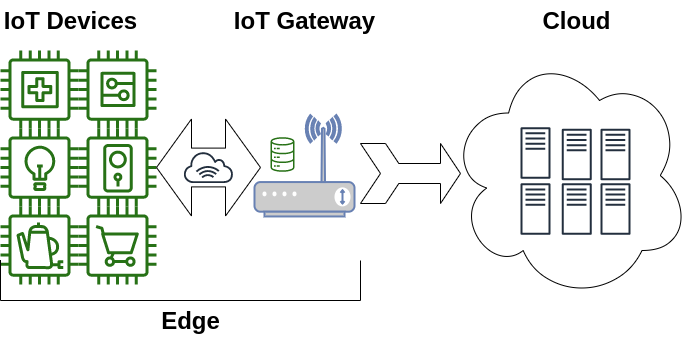
\includegraphics[width=6.5in]{figures/iot_gateway.png}
~\caption{Typical Gateway-based IoT deployment scheme.}
\label{figure1.1}
\end{figure}

Some of the features that could supply the IoT gateway are the following:

\begin{itemize}
  \item communication bridge
  \item data storage, filter and aggregation
  \item device management and configuration
  \item Security 
  \item route data
\end{itemize}

The presence of this Edge Layer facilitates the implementation of collaborative computing across devices, and it helps to apply data management policies. However, this edge layer is not usually rich in computing resources (mainly due to energy consumption limitations), which dramatically limits the approaches and designs that could be implemented to port move computing tasks to the edge. Following the Cloud-oriented approach of hypervisor-based virtualization, it can be proven that it can be cumbersome on these devices~\cite{arxiv:doluikiraly:2018}.
However we will see that this type of approach can be of great help using the proper hypervisor in order to gain the maximum efficiency.

\newpage
\section{Objectives}
\label{makereference1.2}

The main goal of the project is to prove that an IoT gateway using hypervisor-based virtualization reports improvements over an IoT edge environment is able to provide virtual machines capable of using real USB accelerators connected through a low spec motherboard.

Therefore with the purpose of show some results, a virtual appliance has been created running a custom service developed entirely from scratch using new technologies, these areas are highlighted in greater detail in the next chapters. 

With our appliance working, the next milestones are going to be evaluated:

\begin{itemize}
  \item Inference with virtual machines using real USB accelerators
  \item The feature of share real USB accelerators between multiple virtual machines
  \item Dynamic resource allocation including CPU or memory 
\end{itemize}

\subsection{Use case}
\label{makereference1.2.1}
Under the principles previously established it has been defined a use case that allows the appliance development to have a concise scenario in order to achieve better results. The project is aimed at apartments blocks, takes into account a modern building in which every house can be considered an smart house, having a large quantity of sensors across the area.

An external provider or a neighbourhood community wants to take advantage of EpFiot. That provider will be referred as client:
\begin{itemize}
  \item A low cost board will be deployed in base building of flats/apartments as an IoT Gateway with Epfiot appliance installed.
  \item Client will provide each apartment with sensors (temperature, humidity, camera, gas...).
  \item Epfiot appliance will have GPU accelerators physically connected through usb ports.
  \item Epfiot appliance will provide a service to the client allowing the spawn of customized vms that have direct access to the gpu accelerators.
  \item Client will be able to configure sensors using epfiot.
  \item Client will have full access and management for the vms and he will be able to allocate some resources including the usb accelerators.
  \item Sensors will generate data, instead of sending this data directly to internet, a proper vm could receive the data and use a accelerator for perform inference.
  \item Results could be stored in epfiot or another application in a low latency context.
\end{itemize}

Figure ~\ref{figure1.2} shows a representation of the case listed above.

\begin{figure}[h]%t=top, b=bottom, h=here
% \centering
    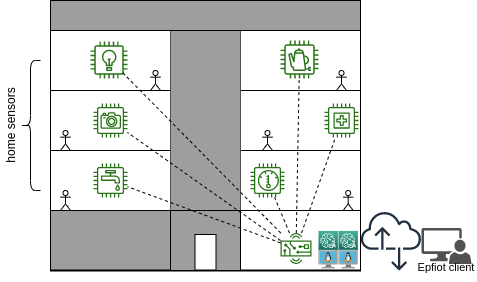
\includegraphics[width=6.5in]{figures/use_case.png}
~\caption{epfiot use case example}
\label{figure1.2}
\end{figure}

\newpage
\section{Document Organization}
\label{makereference1.3}

This document contains 7 chapters described as follow:

\begin{itemize}
  \item \textbf{Chapter 1, Introduction:} This chapter introduces a set of conceptual definition that is going to be mentioned along the document. This chapter also displays the complete project 's purpose through the explanation of its motivations and goals.
  \item \textbf{Chapter 2, State of the Arts:} This section displays the current state of Edge computing from a infrastructure point of view, discussing the underlyng technologies together with the advantages and disadvantages of each option. Finishing by a brief overview of related projects.
  \item \textbf{Chapter 3, Development Environment:} A list of the main technologies used for Epfiot will be enumerated, underlining what kind of utility is used for the project. Hardware and requirements are also discussed in this chapter.
  \item \textbf{Chapter 4: Architecture}: The chapter describes the overall architecture of Epfiot, reviewing every component and how they are connected between each other. 
  \item \textbf{Chapter 5: Features:} This part explains in detail the features of the project, end-user's functionalities are listed.   
  \item \textbf{Chapter 6: Results:} This section is about showing the final results that are obtained with the Epfiot application running. 
  \item \textbf{Chapter 7: Conclusions and Future Work:} Finally a brief summary of the project commenting what kind of implications it has and how to improve the current status of the project in a near future. 
\end{itemize}

%Here's an example of a citation to a single
%work.~\citet{CT:Weiner:1999} It's also possible to make multiple
%citations.~\citet{CT:Phillips:1985, ARP:Loy:1974}
